\documentclass[a4paper,11pt]{article}
\usepackage[a4paper, left=1.5cm, right=1.5cm, top=2.0cm, bottom=3.5cm, headsep=1.2cm]{geometry}
\usepackage{polski}
\usepackage{amssymb}
\usepackage[utf8]{inputenc}
\prefixing
\usepackage{latexsym}
\usepackage{graphicx}
\usepackage{hyperref}
\author{Klaudia Balcer}
\title{Uogólnienia Regresji Poissona}
\frenchspacing
\begin{document}
\maketitle
\begin{center}
Zaawansowane Modele Liniowe

Raport 3 
\end{center}
\tableofcontents


\includegraphics[scale=1]{/home/kabalcer/Dokumenty/licencjat/Zipf_est_plots/Rplot1.png} 

\includegraphics[scale=1]{/home/kabalcer/Dokumenty/licencjat/Zipf_est_plots/Rplot2.png} 

\includegraphics[scale=1]{/home/kabalcer/Dokumenty/licencjat/Zipf_est_plots/Rplot3.png} 

\includegraphics[scale=1]{/home/kabalcer/Dokumenty/licencjat/Zipf_est_plots/Rplot4.png} 

\includegraphics[scale=1]{/home/kabalcer/Dokumenty/licencjat/Zipf_est_plots/Rplot5.png} 

\includegraphics[scale=1]{/home/kabalcer/Dokumenty/licencjat/Mandelbrot_est_plots/Rplot1.png} 

\includegraphics[scale=1]{/home/kabalcer/Dokumenty/licencjat/Mandelbrot_est_plots/Rplot2.png} 

\includegraphics[scale=1]{/home/kabalcer/Dokumenty/licencjat/Mandelbrot_est_plots/Rplot3.png} 

\includegraphics[scale=1]{/home/kabalcer/Dokumenty/licencjat/Mandelbrot_est_plots/Rplot4.png} 

\includegraphics[scale=1]{/home/kabalcer/Dokumenty/licencjat/Mandelbrot_est_plots/Rplot5.png} 

\section{Graficzna analiza danych}

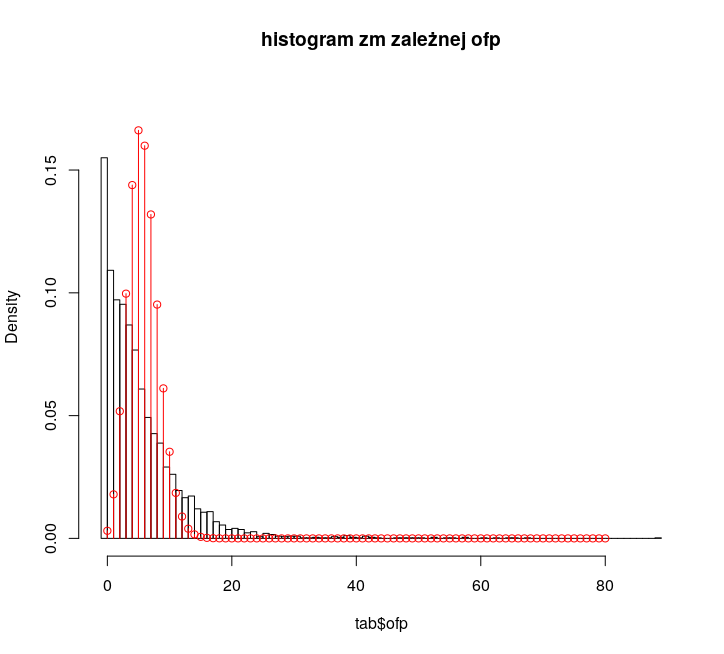
\includegraphics[scale=1]{Rplot0.png} 

Do histogramu dołożyłam funckję prawdopodobieństwa rozkładu Poissona z parametrem $\lambda$ równym średniej próbkowej zmiennej objaśniającej (wyrysowane kolorem czerwonym).  Dane wyraźnie się nie dopasowały -- ciążą na lewo.
Dostrzegamy wyraźnie większą niż dla rozkładu Poissona liczbę obserwacji o zmiennej zależnej równej zero, czyli zjawisko inflacji w zerze. 

Boxploty pokazują wyraźną korelację między zmiennymi ofp a zmienną hosp, health i numchron. Warto jednak zwrócić uwagę, że nawet jeśli mediany utrzymują się na podobnym poziomie dla równych wartości predykatora, zmienia się symetryczność jego rozkładu. Może to świadczyć o związku predykatora z inflacją w zerze, a co za tym idzie,  może istnieć niewidoczna na boxplotach korelacja również w modelu count. Toteż o odrzucaniu jakichkolwiek  zmiennych będę decydować na podstawie testów, po analizie  graficznej nie mam podstaw  by podjąć jednoznaczą decyzję o odrzuceniu którejkolwiek zmiennej. 

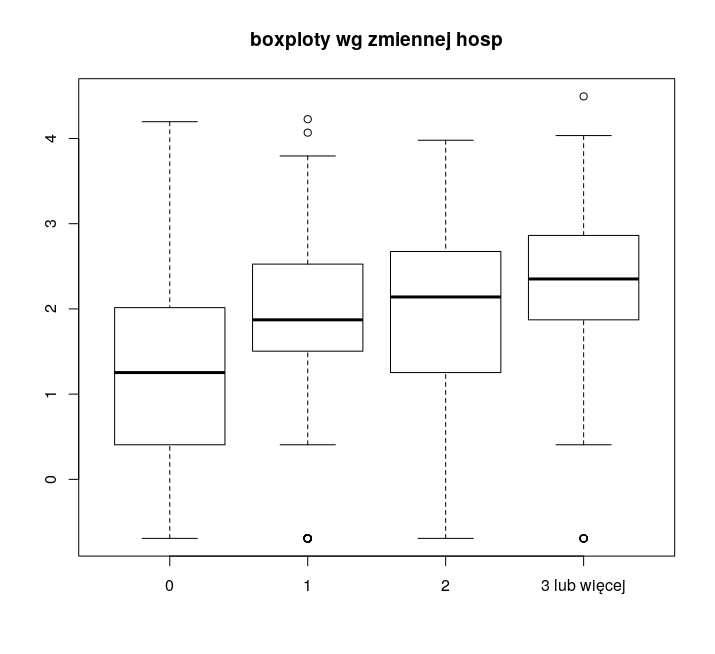
\includegraphics[scale=.45]{Rplot2.png} 
\includegraphics[scale=.45]{Rplot3.png} 

\includegraphics[scale=.45]{Rplot4.png} 
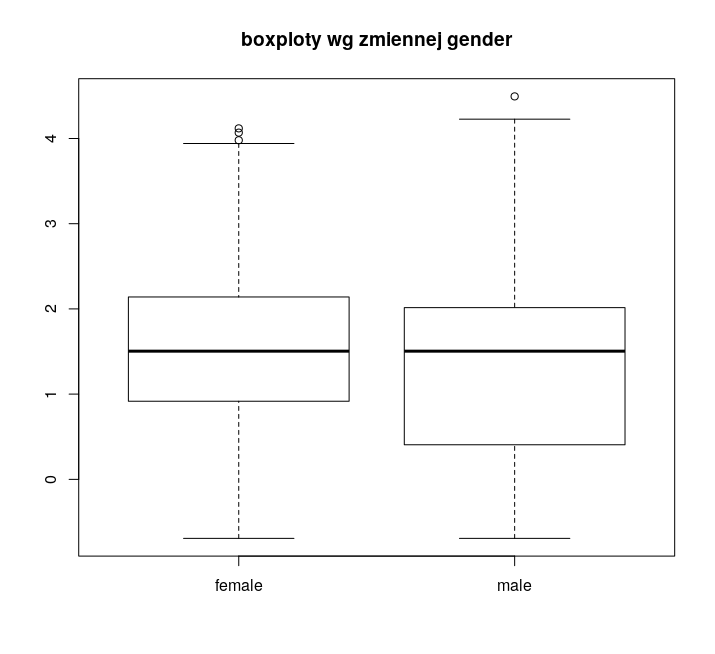
\includegraphics[scale=.45]{Rplot5.png}
 
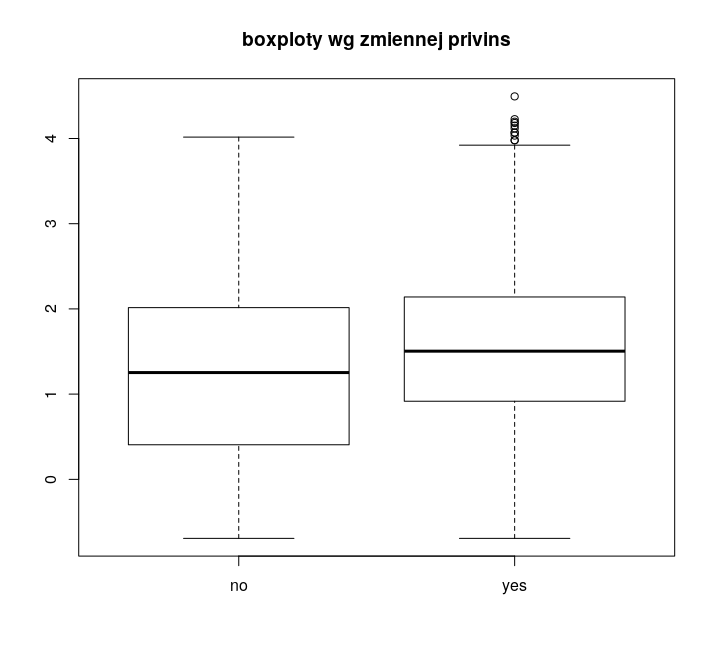
\includegraphics[scale=.45]{Rplot6.png} 
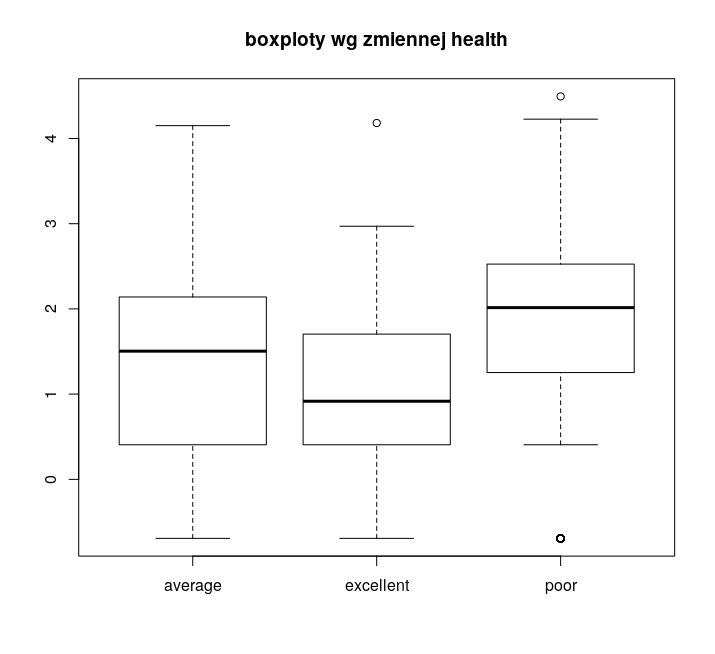
\includegraphics[scale=.45]{Rplot7.png} 

\section{Modele uogólniające regresję Poissona}

Regresja Poissona wymaga rozszerzenia, gdy niespełnione jest założenie o równości wariancji i wartości oczekiwanej (własność rozkładu Poissona) bądź gdy mamy dużo więcej wyników \textit{zero} niż można by się spodziewać po rozkładzie Poissona. Zjawiska te nazywamy odpowiednio nadmierną dyspersją i inflacją w zerze. 

Rozkład używany przy nadmiernej dyspersji wiąże się z wprowadzeniem drugiego  parametru odpowiadającego za zwiększenie wariancji.  Przy modelowaniu inflacji  w zerze budujemy dwa modele --  jeden z rozkładem dwumianowym, jeden z regresji Poissona (w  razie potrzeby z rozkładów modelujących za dużą wariancję).  Wówczas zero może się pojawić jako konsekwencja wyniku z obu zastosowanych rozkładów  (zawsze gdy rozkład dwupunktowy daje 0 lub jeśli uzyskamy 1 z rozkładu dwupunktowego,  to też może pojawić się zero z prawdpopodobieństwem zadanym przez \textit{count model}). Można też zbudować model z barierą. Zasadniczo różni się on od modeli ZIPR//ZINPR//ZIGPR  tym, że o tym czy otrzymamy zero decyduje wyłącznie rozkład dwupunktowy. Jeśli rozkład dwupunktowy da nam 1, na pewno otrzymamy dodatnią wartość predykatora, a gęstość rozkładu w modelu liczącym jest odpowiednio przeskalowana, by nie obejmowała zera.  

\subsection{Funkcje prawdopodobieństwa zmiennej objaśnianej w kolejnych modelach}



\paragraph{Regresja Poissona}

$$P(Y=k|\lambda) = \frac{e^{-\lambda} \lambda^{k}}{k!} $$ 

\paragraph{Regresja ujemna dwumianowa} (stosowane przy nadmiernej dyspersji)

$$ P(Y=k|\mu, \alpha) = \frac{\Gamma(k+ \alpha^{-1})}{\Gamma(k+1)\Gamma(\alpha^{-1})} \Bigg( \frac{\alpha^{-1}}{\alpha^{-1}+\mu} \Bigg)^{\alpha^{-1}} \Bigg( \frac{\mu}{\alpha^{-1}  + \mu}  \Bigg)^{k} $$

Przy $\alpha \rightarrow 0 $ mamy $NB(\mu, \alpha) \rightarrow Pois(\mu)$. 

\paragraph{Regresja z uogólnionym rozkład Poissona} (stosowane przy nadmiernej dyspersji)

$$ P(Y=k|\mu, \phi) = \frac{1}{k!} \Big(\mu+ (\phi -1)k\Big)^{k-1} \phi^{-k} exp\Big(-\frac{1}{\phi}(\mu +  (\phi -1)k)   \Big) $$

Dla $\phi =  1$ rozkład ten pokrywa  się z rozkładem Poissona. 

\paragraph{Zero Inflated Regression}

Funkcje prawdopodobieństwa wszystkich poznanych i użytych w tym sprawozdaniu rozkładów tworzone są  wg wzorca:  

$$ P(Y=k|\mu, \phi, \pi) = \left\lbrace \begin{array}{ll}
\pi + (1-\pi)f(0,\mu, \phi) & k=0 \\
(1-\pi)f(k,\mu, \phi)& k = 1, 2, \ldots \\
\end{array}  $$ 

Gdzie $f(k,\mu, \phi)$ jest funkcją prawdopodobieństwa zmiennej w modelu bez inflacji z zerze. W ten sposób uzyskujemy modele ZIPR, ZIGPR, ZINBR z funkcjami prawdopodobieństwa jak powyżej. Możemy wymodelować sytuację, kiedy zachodzą zarówno nadmierna dyspersja i inflacja w zerze lub tylko inflacja  w zerze.  

\paragraph{Model z barierą}

$$ P(Y=k|\mu, \phi, \pi) = \left\lbrace \begin{array}{ll}
f_{zero}(0,\mu, \phi) & k=0 \\
(1- f_{zero}(0,\mu, \phi))\frac{f_{count}(k,\mu, \phi)}{1- f_{count}(0,\mu, \phi)}& k = 1, 2, \ldots \\
\end{array}  $$ 


\subsection{Implementacja}

\paragraph{Zbudowane modele:}

\begin{verbatim}
poiModel <- glm(ofp~hosp+health+numchron+gender+school+privins, data = tab, 
	family = "poisson")
	
negbinModel <- glm.nb(ofp~hosp+health+numchron+gender+school+privins, data = tab)

r_zipr <- zeroinfl(ofp~hosp+health+numchron+gender+school+privins|
	hosp+numchron+gender+school+privins, data = tab, dist="poisson")
	
r_poiHurdle <- hurdle(ofp~hosp+health+numchron+gender+school+privins|
	hosp+numchron+gender+school+privins, data = tab, dist="poisson")
	
r_negbinHurdle <- hurdle(ofp~hosp+health+numchron+gender+school+privins|
	hosp+numchron+gender+school+privins, data = tab, dist="negbin")
	
r_r_zinbr <- zeroinfl(ofp~hosp+health+numchron+gender+school+privins|
	numchron+gender+school+privins, data = tab, dist="negbin")
\end{verbatim}

Wszystkie modele z inflacją w zerze wymagały redukcji w regresji z rozkładem dwupunktowym. W ZINBR usuwałam dwie zmienne, toteż robiłam to kolejno, testując po każdym kroku. Poparłam te redukcje testami za pomocą statystyki Deviance:

\begin{verbatim}
 > -2 *(logLik(zipr) -  logLik(r_zipr)) < qchisq(0.9, 2)
[1] TRUE
> -2 *(logLik(zinbr) -  logLik(r_r_zinbr)) < qchisq(0.9, 1)
[1] TRUE
> -2 *(logLik(poiHurdle) -  logLik(r_poiHurdle)) < qchisq(0.9, 2)
[1] TRUE
> -2 *(logLik(negbinHurdle) -  logLik(r_negbinHurdle)) < qchisq(0.9, 2)
[1] TRUE
\end{verbatim}

Zbudowałam równeż  model regresji Poissona i model regresji ujemnej dwumianowej z interakcjami. Do wyboru zmiennych użyłam metod krokowych opartych na kryterium Akaike (biblioteka MASS, funckja \textit{stepAIC()}). Użycie metod \textit{both} oraz \textit{backward} dało dużo zmiennych, których testy Studenta wskazywały na brak istotności.  AIC zmieniło się nieznacznie przy uwzględnieniu interakcji (w regresji Poissona poprawa nastąpiła z 35959 na 34979; w  regresji ujemnej dwumianowej zmiana z 24359 na 24356). W związku z tym w dalszej części raportu szczegółowo przedstawię jedynie wyniki dla modeli bez interakcji.  


\begin{verbatim}
stepPoi <- stepAIC(glm(ofp~hosp*health*numchron*gender*school*privins, 
data = tab, family = "poisson"), direction = "backward", steps  = 1000)

stepNegBin <- stepAIC(glm.nb(ofp~hosp*health*numchron*gender*school*privins, 
data = tab), direction = "backword", trace = TRUE,  steps = 1000)

> AIC(stepPoi)
[1] 34978.88
> AIC(stepNegBin)
[1] 24365.67
\end{verbatim}

\pagebreak

\subsection{Wyniki}

%\paragraph{Współczynniki,}  parametry i wartości kryteriów informacyjnych: 

\begin{tabular}{|c|c|c|c|c|c|c|}  \hline


 & Poisson & NegBin &  ZIPR & ZINBR & Poisson z berierą & NegBin z berierą \\ \hline
 
\multicolumn{7}{|l|}{Count model  -- wpółczynniki:} \\ \hline

(Intercept) & 1.028874 & 1.028874 & -0.08102  & 1.193466 & 1.406459 &  1.197699      \\ 
hosp        & 0.164797 &  0.164797 & -0.30330 & 0.201214 & 0.158967 &  0.211898   \\ 
healthexcellent & -0.361993 & -0.361993 & 0.23785 & -0.313540 & -0.303677 &  -0.331861     \\ 
healthpoor  & 0.248307 & 0.248307 & 0.02166 &  0.287190 & 0.253521 & 0.315958    \\ 
numchron    & 0.146639 & 0.146639 & -0.53117  & 0.128955 & 0.101720 &   0.126421    \\ 
gendermale  & -0.112320 & -0.112320 &  0.41527  &  -0.080093 & -0.062247 &   -0.068317       \\ 
school      &  0.026143 & 0.026143  &  -0.05677 & 0.021338 & 0.019078 &  0.020693    \\ 
privinsyes  & 0.201687 & 0.201687 & -0.75294  &  0.126815 & 0.080879 &  0.100172   \\ 
theta  & & 1.2066 &  &  1.4853  &  & 1.3955 \\  \hline 
\multicolumn{7}{|l|}{ Zero model -- wpółczynniki: } \\ \hline
(Intercept) & & &     -0.05937  &  -0.07042  &  0.01594   &  0.01594 \\  
hosp       & & &      -0.30669  &            &  0.31843   &  0.31843     \\ 
numchron  & & &       -0.53972  &  -1.24726  &  0.54783   &  0.54783      \\ 
gendermale   & & &     0.41807  &   0.55586  & -0.41915   & -0.41915     \\ 
school       & & &    -0.05560  &  -0.08394  &  0.05707   &  0.05707     \\ 
privinsyes     & & &  -0.75373  &  -1.24290  &  0.74572   &  0.74572     \\ \hline

\multicolumn{7}{|l|}{Informacje o modelu: } \\ \hline
log-wiarogoność &  -17971.61 &  -12170.55 &  -16135.24 &  -12094.25  & -16136.44   & -12090.07  \\
AIC & 35959.23 & 24359.11 & 32298.49 & 24216.51  & 32300.88  & 24210.14 \\
BIC & 36010.35 & 24416.62 & 32387.96   & 24305.98   &   32390.35   &  24306    \\
liczba zer & 47 & 608 & 682  &  707   &  683   &  683   \\ \hline 

\end{tabular}

\linebreak

Widzimy, że zdecydowanie lepsze parametry mają modele z nadmierną dyspersją (dopiero po wymodelowaniu inflacji w zerze, którą wyraźnie wskazała nam graficzna analiza, można było zbadać czy wariancja w modelu liczącym jest większa istotnie niż wartość oczekiwana). 

Najodpowiedniejszymi modelami są Zero  Inflated Negative Binomial Regression i Negative Binomial Hurdle  Model. Statystycznie się one nie różnią (porównałam je za pomoca statystyki Deviance). Ze względu na charakter danych za najodpowiedniejszy uważam ZINBR. Model z barierą przewiduje, że jeśli wejdziemy w grupę pozytywnego wyniku z testu dwumianowego nie ma możliwości uzyskania zera. Dane mówią o liczbie pobytów  w szpitalu -- brak  pobytów w szpitalu jest możliwy również w przypadku osób, które są w pewien sposób zakwalifikowane do \textit{grupy  ryzyka}.

Bardzo dobre wyniki wykazał również model regresji ujemnej dwumianowej. Wyraźnie widoczna w analizie graficznej inflacja w zerze daje jednak przesłanki, że nie jest on najodpowiedniejszy. 

\pagebreak

\section{Tetsowanie hipotez brzegowych -- statystyki $\chi^{2}$ i $T$ -- symulacja}

Przedstawię rozkłady statystyk w testowaniu:

$H_{0}: \quad $ dane pochodzą z rokładu normalnego

$H_{1}: \quad$ dane pochodzą z rozkładu ujemnego dwumianowego

Test ten przeprowadzamy w oparciu o statystykę Deviance lub o statystykę $T = \frac{\widehat{\alpha}}{\sqrt{Var(\widehat{\alpha})}}$. Przy hipotezie alternatywnej statystyka $T$ ma rozkład standardowy normalny. Przy hipotezie zerowej rozkład na półprostej dodatniej pozostaje bez zmian, natomiast masa probabilistyczna rozrzucona po ujemnej półosi koncentruje się w zerze. 

W poniższych symulacjach przedstawię oprócz rozkładu statystyki T, rozkład estymatora $\widehat{\alpha} = T \cdot Var(\widehat{\alpha})$. Lepiej obrazuje on opisane wyżej własności. 



\subsection{Statystyka $\chi^2$}

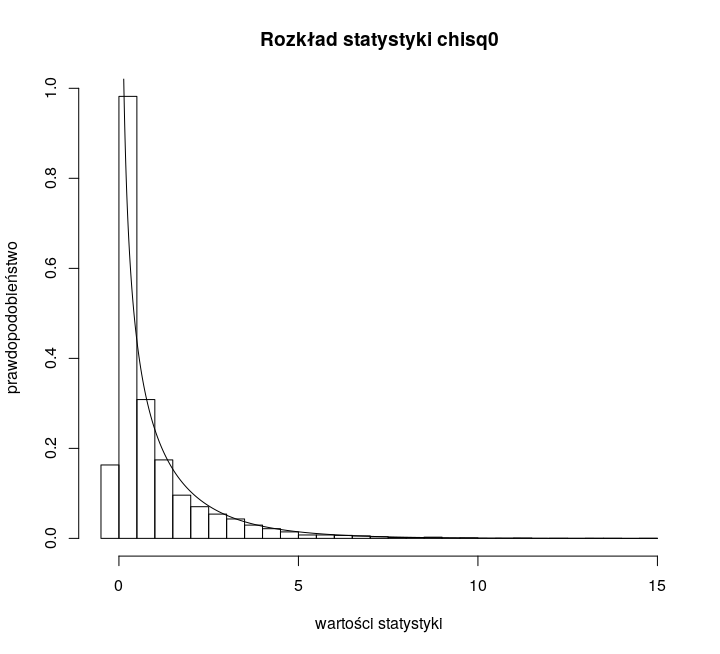
\includegraphics[scale=.3]{Rplot8.png} 
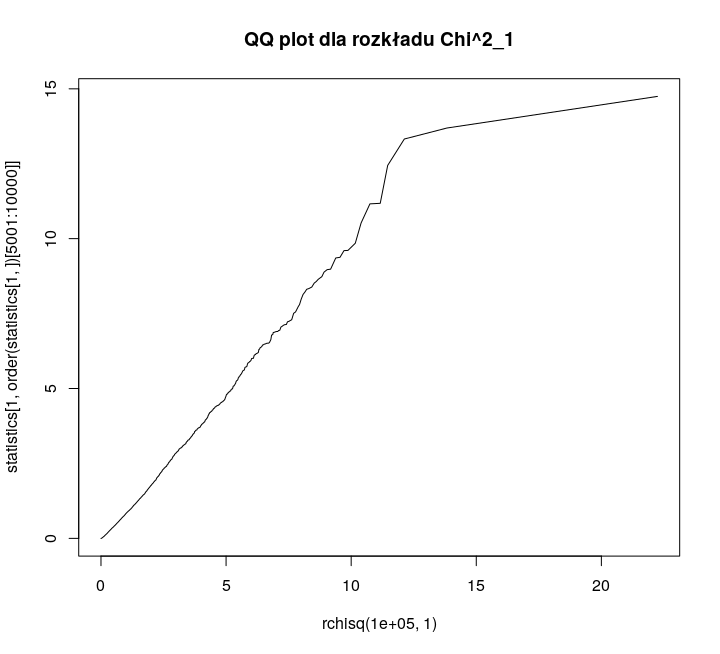
\includegraphics[scale=.3]{Rplot9.png} 
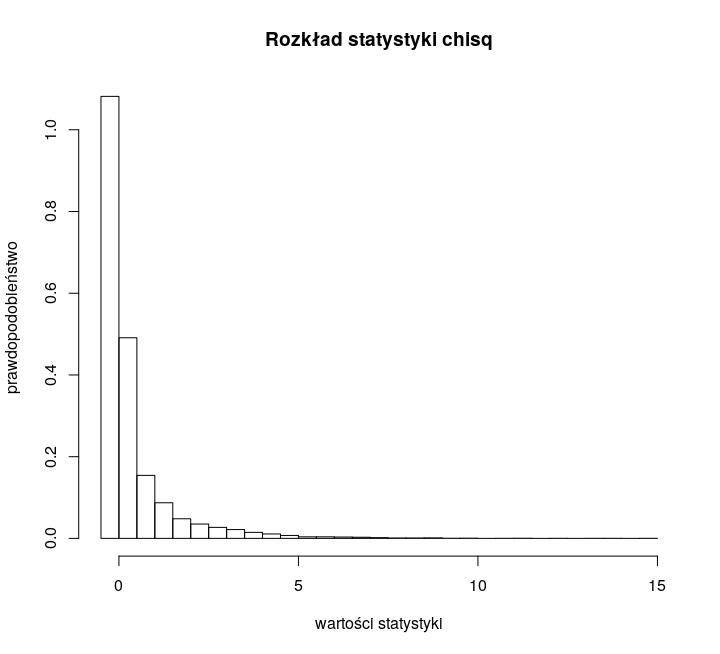
\includegraphics[scale=.3]{Rplot99.png} 

Zaburzenia ze względu na dopasowanie do teoretycznego rozkładu dostrzegamy ze względu na obserwacje odstające. Przy większej próbie z  pewnością wpływ outlierów byłby mniejszy. Pomimo tych odchyleń rozkład dość dobrze dopasował się do teoretycznego.

Po lewej stronie mamy histogram połowy obserwacji (część mieszaniny rozkładu statystyki związana z rozkłądem $\chi^{2}_{1}$)  z dorysowaną odpowiednią gęstością teoretyczną. Po prawej natomiast widzimy rozkład  nazywany $\chi^{2}_{0}$ --  czyli mieszaninę rozkładu skumulowanego w zerze oraz rozkładu  $\chi^{2}_{1}$. 

\subsection{Estymator $\widehat{\alpha}$} 

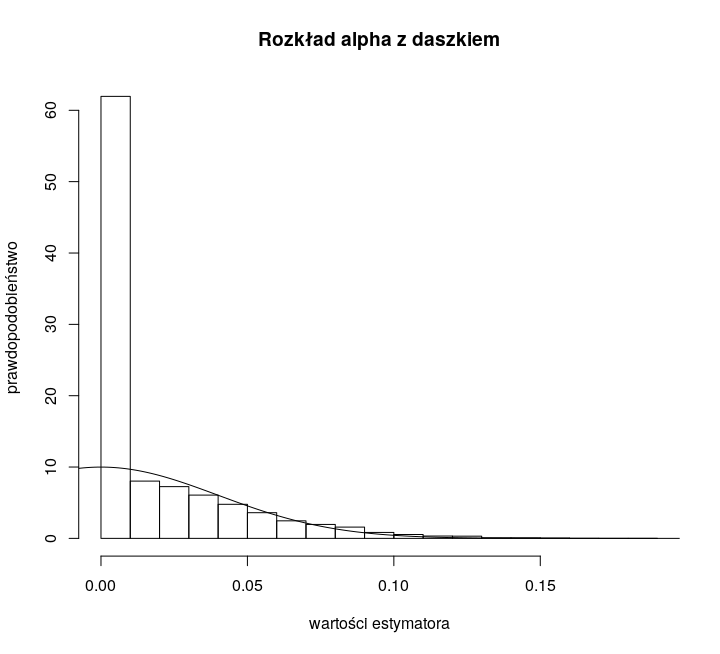
\includegraphics[scale=.3]{Rplot10.png} 
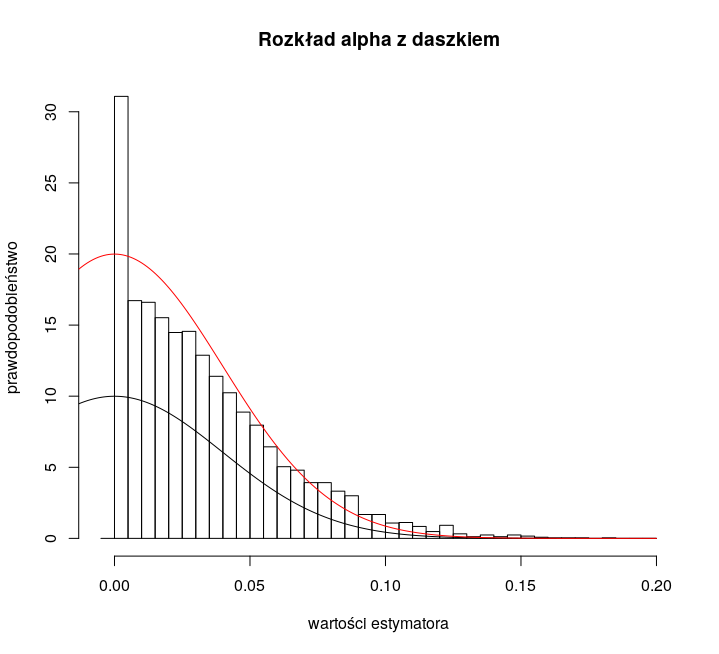
\includegraphics[scale=.3]{Rplot11.png} 
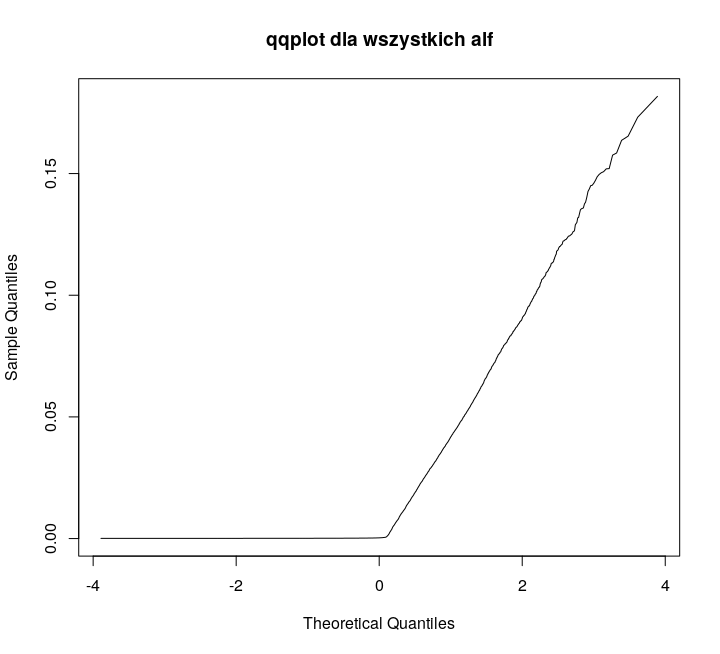
\includegraphics[scale=.3]{Rplot12.png} 

Rozkład estymatora alfa dopasował  się do rozkładu normalnego o wariancji oszacowanej jako iloraz kwantyli rzędu 0.75 z próby wektora alpha (przed odrzuceniem części rozkładu skumulowanej w zerze) przez kwantyl rozkładu standardowego normalnego. Rozkład jest jednostronny, więc dopasowałam do histogramu odpowiednią gęstość przemnożoną przez dwa po odrzuceniu połowy najmniejszych statystyk (linia czerwona na środkowym wykresie). W przypadku nieodrzucenia kumulacji w zerze dopasowuję do histogramu gęstość bez przeskalowania (rysunek po lewej). Wykres kwantylowo-kwantylowy spełnia nasze oczekiwania. Ujemna część rozkładu normalnego dla estymatora alfa skumulowała się w zerze, natomiast kwantyle rzędów wyższych niż 0.5 dla  rozkładu teoretycznego i empirycznego wykazują zależność liniową. 


\subsection{Statystyka T}


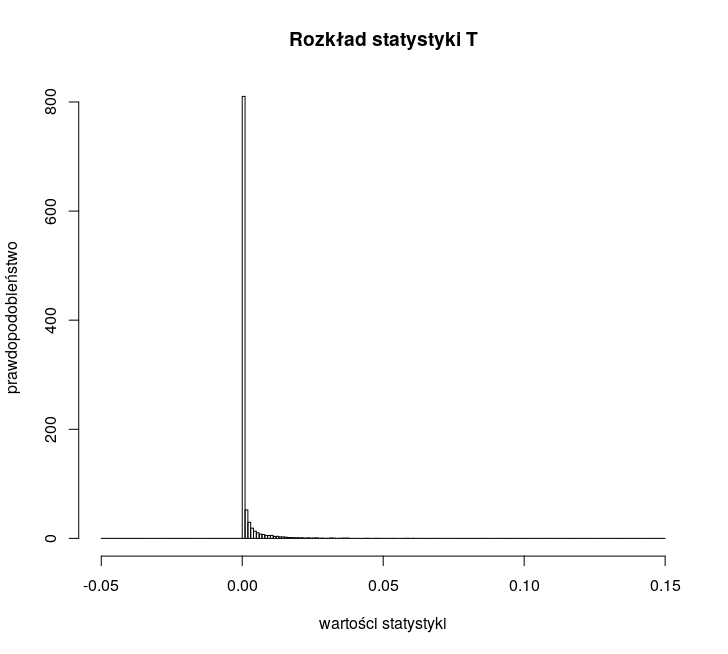
\includegraphics[scale=.3]{Rplot100.png} 
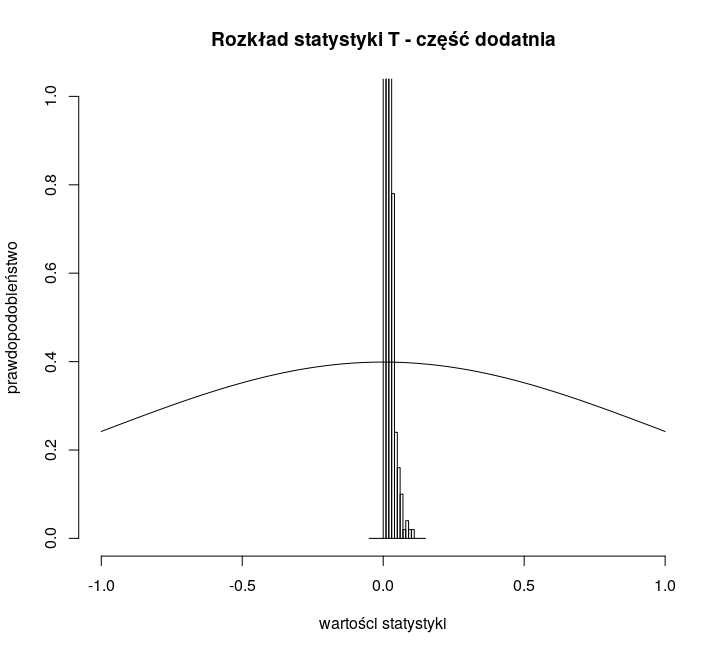
\includegraphics[scale=.3]{Rplot101.png} 
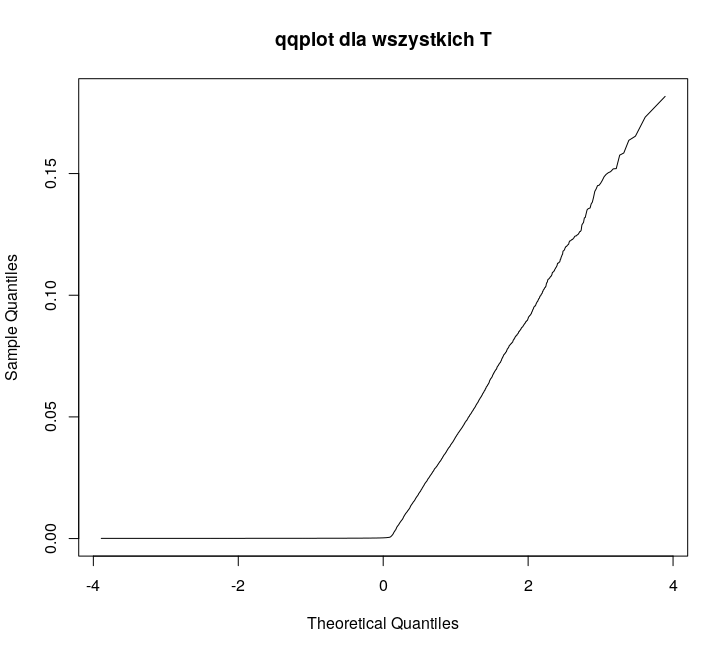
\includegraphics[scale=.3]{Rplot102.png} 

Po lewej histogram z uwzględnieniem argumentu \textit{freq=FALSE}, po lewej histogram po odrzuceniu połowy najmniejszych wartości (odrzucenie masy skoncentrowanej w zerze lub na ujemnej półosi) z dorysowanym fragmentem gęstości rozkładu standardowego normalnego. Znacznie wyraźniej niż dla alf obserwujemy, że w zerze skoncentrowane jest więcej niż połowa masy. Wykres kwantylowo-kwantylowy pokazuje jednak, że rozkład statystyki T zachowuje się tak, jak byśmy się tego spodziewali: połowa masy w zerze i normalność na dodatniej półosi.




\end{document}